\documentclass{article}
\documentclass{bar}
\usepackage{graphicx}
\usepackage[utf8]{inputenc}
\usepackage[fleqn]{amsmath}
\usepackage{titling}
\usepackage{graphicx,wrapfig,lipsum}
\usepackage{amssymb}
\usepackage{listings}
\usepackage{mathtools}
\usepackage[font=small,labelsep=none]{caption}
\usepackage{hyperref}

\setlength{\droptitle}{-10em}
\setlength\parindent{0pt}

\title{Project 1 - FYS3150}\vspace{-3ex}
\author{Benedicte Allum Pedersen, Emil Helland Broll\\ Fredrik Oftedal Forr}
\date{\vspace{-5ex}}

\begin{document}
\maketitle

\subsection*{Introduction}
In this report we will address several ways of solving linear equations. The methods we will use are the Thomas algorithm and LU decomposition. The Thomas algorithm is found through the solution of the one-dimensional Poisson equation with Dirichlet boundary conditions, rewritten as a linear algebra problem, which we will explain later this report. To perform the LU decomposition, the linear algebra package Armadillo for C++ was used. The links to the GitHub repository for our programs are in the appendix.

\vspace{0.3cm}

The equation we solve to arrive at the Thomas algorithm is the Poisson's equation, which is a classical equation from electromagnetism. In three dimensions the equation is as follows:
\begin{equation*}
\nabla^2 \Phi = -4\pi \rho (\mathbf{r}).
\end{equation*}

Here $\Phi$ is the electrostatic potential generated by a localized charge distribution $\rho (\mathbf{r})$. If $\Phi$ and $\rho (\mathbf{r})$ are spherical symmetrical, and we do the substitution $\Phi(r)= \phi(r)/r$, the equation simplifies to:
\begin{equation*}
\frac{d^2\phi}{dr^2}= -4\pi r\rho(\mathbf{r}).
\end{equation*}

If we let $f(\mathbf{r}) = -4\pi r \rho (\mathbf{r})$, and consider what happens when $\phi\rightarrow u$ and
$r\rightarrow x$, the general one-dimensional Poisson equation will read:
\begin{equation*}
-u''(x) = f(x).
\end{equation*}

\subsection*{Project 1 a)}

\noindent By solving the one-dimensional Poisson equation with Dirichlet boundary conditions, we can rewrite the solution as a set of linear equations.\\

\noindent We let the discretized approximation to $u$ be defined as $v_i$. The second derivative of $u$ is then defined as:
\[
&-\frac{v_{i+1}+v_{i-1}-2v_i}{h^2} = f_i
\]
where $h$ is the step length, defined as $h=1/(n+1)$, and $f_i = f(x_i)$.
We can rewrite this equation to a set of linear equations like this:
\begin{flalign*}
   &-\frac{v_{i+1}+v_{i-1}-2v_i}{h^2} = f_i\\
   &-(v_{i+1}+v_{i-1}-2v_i) = f_ih^2\\
   &2v_i -v_{i+1}-v_{i-1}=f_ih^2
\end{flalign*}
Which expands to
\begin{flalign*}
  2v_1 - v_0 - v_2 &= f_1h^2\\
  2v_2 - v_1 - v_2 &= f_2h^2\\
  &\vdots\\
  2v_n - v_{n-1} - v_n+1 &= f_3h^2\\
\end{flalign*}
The boundary conditions give us $v_{n+1}=u(1)=0$ and $v_0=u(0)=0$. We also introduce $f_ih^2 = g_i$. We can then simplify the above linear equations into a matrix:
\begin{flalign*}
  \begin{bmatrix}
    2 & -1 & 0 &\dots & 0 & 0\\
    -1 & 2 & -1 & \dots & 0 & 0\\
    0 & -1 & 2 & \dots & 0 & 0 \\
    \vdots & \vdots & \vdots & \ddots & \vdots & \vdots \\
    0 & 0 & 0 &\dots& 2 & -1\\
    0 & 0 & 0 &\dots& -1 & 2
  \end{bmatrix}
  \begin{bmatrix}
    v_1\\
    v_2\\
    v_3\\
    \vdots\\
    v_{n-1}\\
    v_n
  \end{bmatrix} =
  \begin{bmatrix}
    g_1\\
    g_2\\
    g_3\\
    \vdots\\
    g_{n-1}\\
    g_n
  \end{bmatrix}
\end{flalign*}


\subsection*{Project 1 b)}
A tridiagonal (n x n)-matrix can be rewritten in terms of one-dimensional vectors $a$ and $c$ of length $n-1$ and $b$ of length $n$:
\begin{flalign*}
  \mathbf{A}=\begin{bmatrix}
    b_1 & c_1 & 0 &\dots & \dots & 0 \\
    a_1 & b_2 & c_2 & \dots & \dots & 0 \\
    0 & a_2 & b_3 & c_3 & \dots \dots & 0  \\
    \vdots & \vdots & \vdots & \ddots & \vdots & \vdots \\
    0 & 0 &\dots& a_{n-2} & b_{n-1} & c_{n-1}\\
    0 & 0 &\dots& \dots & a_{n-1} & b_{n}
  \end{bmatrix}
\end{flalign*}

To solve the problem $Ax=b$, we first perform a forward substitution. We can develop a general algorithm for the forward substitution of tridiagonal matrices:

\begin{flalign}
  &b_1v_1 + c_1v_2 = \tilde{g}_1\\
  &a_1v_1 + b_2v_2 + c_2v_3 = \tilde{g}_2\\
  &a_2v_2 + b_3v_3 + c_3v_4 = \tilde{g}_3\\
  &\vdots \notag\\
  &a_{n-1}v_{n-1} + a_nv_n = \tilde{g}_n
\end{flalign}
Multiplying equation (1) with $\frac{a_1}{b_1}$:\\
\begin{center}
  $a_1v_1 + \frac{a_1c_1}{b_1}v_2 = \tilde{g_1}\frac{a_1}{b_1} $\\
\end{center}
\vspace{0.3cm}

\noindent We can then subtract equation (1) from equation (2):\\
\begin{flalign*}
  a_1v_1- a_1v_1 + b_2v_2 - \frac{a_1c_1}{b_1}v_2 + c_2v_3 &= g_2 - g_1\frac{a_1}{b_1}\\
  \left(b_2 - \frac{a_1c_1}{b_1} \right)v_2 + c_2v_3 &= g_2 - g_1\frac{a_1}{b_1}\\
  \tilde{b}_2v_2 +c_2v_3 &= \tilde{g}_2
\end{flalign*}

\noindent The resulting general expressions are as follows:
\begin{flalign*}
  \begin{aligned}
    \tilde{b}_i = b_i - \frac{c_{i-1}a_{i-1}}{\tilde{b}_{i-1}}
  \end{aligned},
  \qquad \qquad
  \begin{aligned}
    \tilde{g}_i = g_i - g_{i-1}\frac{a_{i-1}}{\tilde{b}_{i-1}}
  \end{aligned}
\end{flalign*}
Where $\tilde{b}_1 = b_1$ and $\tilde{g}_1 = g_1$\\

\noindent We can then perform a backward substitution to compute the vector $\hat{u}$. This has the general expression:\\
\begin{flalign*}
  v_i = \frac{\tilde{g}_i - a_i v_{i+a}}{\tilde{b}_i}
\end{flalign*}


We have implemented the above algorithms in our C++-program and used that to solve problems with the matrix from 1a) of the sizes 10 x 10, 100 x 100 and 1000 x 1000. The results are showed in Figure 1. By reducing the problem by only using the vectors $a, b$ and $c$, we save memory, and the total number of floating points operations for the bacward and forward substitution will be $O(9n)$.

\begin{figure}[hbt]
\begin{center}
    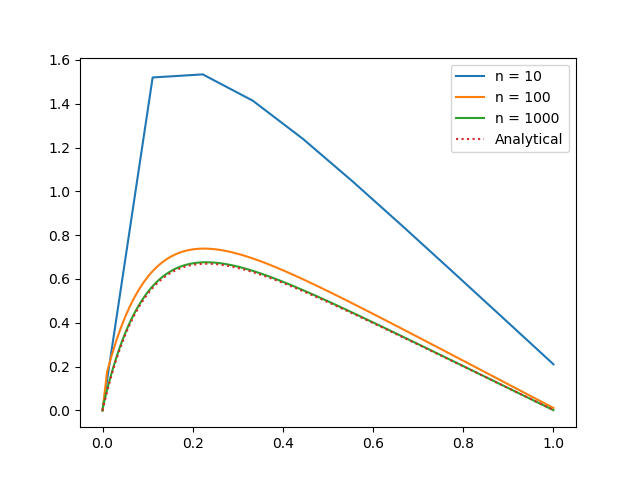
\includegraphics[width=\textwidth]{plot1b.png}
    \caption{: Numerical plot for different values of n compared to an analytical plot for the soulution of the Poisson equation.}
    \label{fig:plot1b}
\end{center}
\end{figure}


\subsection*{Project 1 c)}

For a general solution, the matrix now has identical elements along the diagonal and identical values for the non diagonal elements, visualised below, with $a=-1$ and $b=2$:

\begin{flalign*}
  \begin{bmatrix}
    b & a & 0 &\dots & 0 & 0\\
    a & b & a & \dots & 0 & 0\\
    0 & a & b &  \dots & 0 & 0 \\
    \vdots & \vdots & \vdots & \ddots & \vdots & \vdots \\
    0 & 0 & 0 &\dots& b & a\\
    0 & 0 & 0 &\dots& a & b
  \end{bmatrix}
\end{flalign*}

We then develop an algorithm for the forward substitution in the same way as earlier. Here $\tilde{b}_1 = b = 2$ and the algorithm will run with $i$ starting from 2 and going up to $n$.

\begin{flalign*}
  \begin{aligned}
    \tilde{b_i} &= b - \frac{a^2 + (i-2)}{b + (i-2)} \\
    &= 2 - \frac{i-1}{i}
  \end{aligned},
  \qquad \qquad
  \begin{aligned}
    \tilde{g_i} &= g_i - \frac{a}{\tilde{b}_{i-1}}g_{i-1}\\
    &= g_i + \frac{g_{i-1}}{\tilde{b}_{i-1}} \\
  \end{aligned}
\end{flalign*}

where $\tilde{b}_1 = b$ and $\tilde{g}_1 = g$.

\vspace{0.2cm}

Likewise, the algorithm for the backward substitution will be:

\begin{flalign*}
  \begin{aligned}
    u_i &= \tilde{g}_i - \frac{a}{\tilde{b}_i} v_{i+1}\\
    &= \tilde{g}_i + \frac{v_{i+1}}{\tilde{b}_i}
  \end{aligned},
\end{flalign*}

The number of floating points for this special case is $O(7n)$. Because of this, we can assume this algorithm will be faster than the general tridiagonal matrix in task b). The CPU time for the two algorithms also shows this as the general matrix took 0.028154 seconds while the special case took 0.024463 seconds for $n = 10^6$.


\subsection*{Project 1 d)}
To compute the relative error in the data set for $i = 1,...,n$ we set up:
\[
\epsilon_i = log_{10}(|\frac{v_i - u_i}{u_i}|)
\]

The maximum values for the relative errors for the matrix in task b) are represented in table 1 below. For $n=10^7$ the error is approching zero (resulting in NaN-values), thus the error is decreasing when $n$ is increasing.

\begin{table}[h!]
  \begin{center}
    \caption{ : Relative errors for the general tridiagonal matrix.}
    \label{tab: table1}
    \begin{tabular}{l|r}
      \textbf{n} & \textbf{Max error}\\
      10 & 0.301744 \\
      100 & 0.0374884  \\
      1000 & 0.00384884 \\
      10^7 &   \approx{0}  \\
    \end{tabular}
  \end{center}
\end{table}}

\subsection*{Project 1 e)}

The LU decomposition uses approximately $\frac{2}{3}n^3$ floating points operations to solve a set of linear equations. The differences in the execution time for the LU decomposition and the Thomas algoritm are showed below in Table 2. If we try to run the LU decomposition for a matrix of the size $10^5$ x $10^5$, we get an error message that tells us that the matrix is too large. We can run matrixes on this size with the forward and backward substitutions, so this shows that the LU decomposition is a prossess that requires more from the computer than the Thomas algoritm does.

\begin{table}[h!]
  \begin{center}
    \caption{ : Execution time in seconds for solving linear equations with the LU decomposition and the Thomas algortihm.}
    \label{tab:LU}
    \begin{tabular}{c|c|c}
      \textbf{Size of matrix} & \textbf{LU decomposition (sec)} & \textbf{Thomas algoritm (sec)}\\
      10 x 10 & 0.000114 & 2 x 10^{-6} \\
      100 x 100 & 0.001317 & 7 x 10^{-6}\\
      1000 x 1000 & 0.440127 & 2.4 x 10^{-5} \\
    \end{tabular}
  \end{center}
\end{table}}



\subsection*{Comments}
Our group thought the first exercise of this project was a bit hard to get started with. A suggestion is to split excersises like this into several parts so it will be easier to get started. When we solved exercise a) the rest of the project went a lot smoother.

\subsection*{Appendix}


\href{{https://github.com/emmernme/MENA-Compfys/blob/master/Project%201/}}{Link to the GitHub repository}

\end{document}
